%%%%%%%%%%%%%%%%%%%%%%%%%%%%%%%%%%%%%%%%%%%%%%%%%%%%%%%%%%%%%%%%%%%%%%%%%%%%%%%
\chapter{Fluidi non newtoniani}\label{chp:NonNewton}
%%%%%%%%%%%%%%%%%%%%%%%%%%%%%%%%%%%%%%%%%%%%%%%%%%%%%%%%%%%%%%%%%%%%%%%%%%%%%%%
I materiali polimerici non possiedono comportamento newtoniano.
Possiamo definire come "newtoniano" un fluido per il quale:
\begin{description}
\item[Fluido newtoniano] la viscosità dipende unicamente da temperatura e pressione: $\eta = \eta(T,p)$
\end{description}

Una prima relazione che lega la viscosità a temperatura e pressione può essere quella di \textit{Arrhenius}:
\begin{equation}
\eta = \eta_t e^{\frac{\Delta E}{R}\left(\frac{1}{T}-\frac{1}{T_0}\right)} %
e^{\beta \left(p - p_0\right)}
\label{eqn:Arrhenius}
\end{equation}
Resta evidente come:
\begin{itemize}
\item Se $p \uparrow\uparrow$ allora $\eta \uparrow\uparrow$.
\item Se $T \uparrow\uparrow$ allora $\eta \downarrow\downarrow$. 
\end{itemize}

Nello specifico, i fluidi non newtoniani presentano delle così dette \textbf{deviazioni} dal comportamento del fluido newtoniano.
Ora verranno elencate e poi approfondite nello stesso ordine.

\begin{enumerate}
\item La viscosità dipende dalle condizioni di flusso, in particolare dalla velocità di deformazione.
\item Possono esserci effetti di sforzo normale.
\item Possono esserci effetti di viscoelasticità.
\item Possono esserci effetti di plasticità: ovvero fenomeni di snervamento.
\item Gli effetti sono conseguenze del tempo: \textbf{tissotropia}.
\end{enumerate}

\section{Condizioni di flusso}
Come accennato in precedenza, una deviazione dal comportamento di fluido newtoniano può essere quella della dipendenza dalle condizioni di flusso alle quali il fluido viene sottoposto.
In particolare i fluidi non newtoniani dipendono fortemente dalla velocità di deformazione $\dot{\gamma}$.
Perciò, vale:
\begin{equation}
\eta = \eta(\dot{\gamma})
\label{eqn:viscNonNewt}
\end{equation}
Funzione che lega la viscosità con la velocità di deformazione.
Siccome lo \textbf{sforzo di taglio} vale, sia per fluidi newtoniani che non:
\begin{equation}
\tau = \eta \dot{\gamma}
\label{eqn:sforzoTaglio}
\end{equation}
Da cui, sostituendo la \eqref{eqn:viscNonNewt} alla \eqref{eqn:sforzoTaglio} ne risulta:
\begin{equation}
\tau = \eta(\dot{\gamma}) \dot{\gamma}
\label{eqn:taglioNonNewt}
\end{equation}

\begin{figure}
\centering
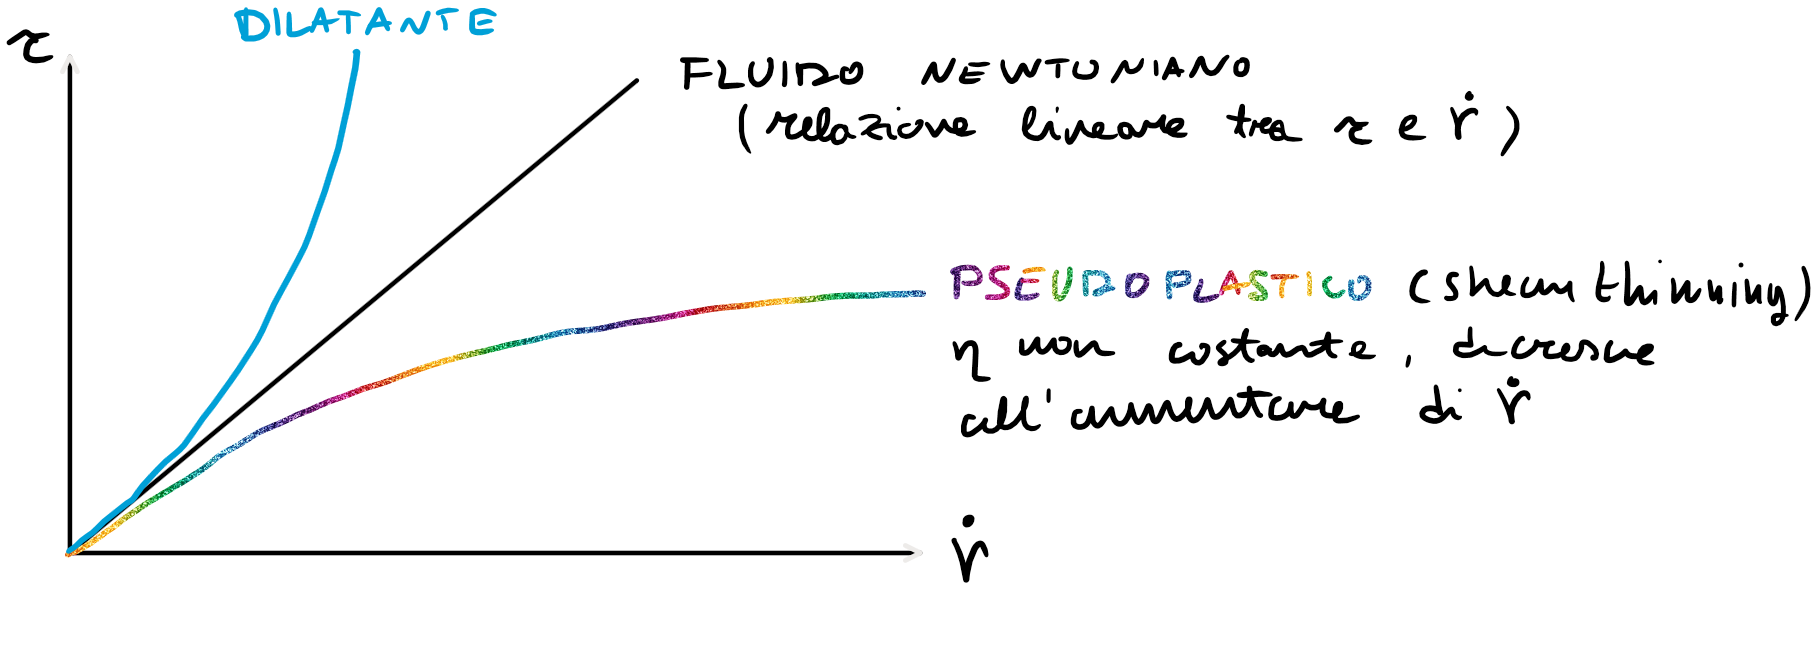
\includegraphics[width = \textwidth]{gfx/TaglioNonNewt}
\caption{Andamento dello sforzo di taglio per diversi fluidi}
\label{fig:TaglioNonNewt}
\end{figure}

Dal grafico \ref{fig:TaglioNonNewt} si può dedurre che:
all'aumentare dello sforzo di taglio il fluido si assottiglia (cioè ha comportamento \textbf{pseudo-plastico} e $\eta$ diminuisce).
Quasi tutti i materiali plastici hanno comportamento pseudo-plastico. Con $\eta$ indipendente dal tempo.
Se $\dot{\gamma}$ aumenta, significa che il fluido di assottiglia sempre di più perché viene speso molto sforzo di taglio per deformare l'oggetto. In generale viene considerato un vantaggio.

Per un fluido polimerico, si può tracciare un comportamento del tipo \ref{fig:PesudoPlastico}.

\begin{figure}
\centering
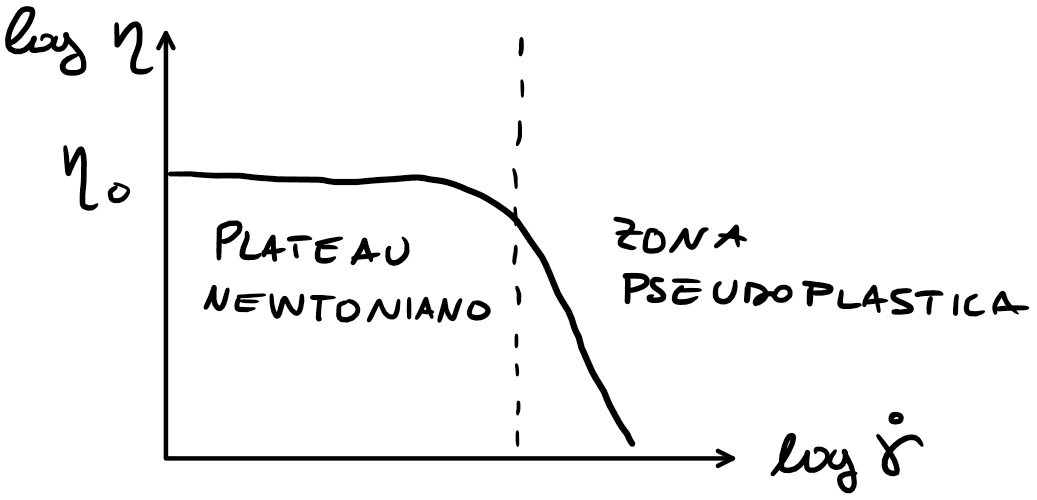
\includegraphics[width = 0.7\textwidth]{gfx/PseudoPlastico}
\caption{Comportamento di un fluido polimerico}
\label{fig:PesudoPlastico}
\end{figure}

\section{Effetti di sforzo normale e viscoelasticità}
\subsection{Sforzo normale}
Se al fluido, all'interno di un qualsiasi contenitore, viene applicato uno sforzo esterno, questo risale grazie ad un movimento di rotazione circonferenziale provocato dall'aderenza.
A livello circonferenziale, le catene polimeriche sono sollecitate a trazione. Tuttavia, nel corso del tempo esse tenderanno a ritornare allo stadio iniziale di gomitolo statistico, esercitando una pressione sull'elemento rotante. Creando così aderenza.
Questo viene anche chiamato \textbf{effetto Poisson}.

\subsection{Viscoelasticità}
Viene detto \textbf{effetto Barus} o di \textbf{rigonfiamento dell'estruso}.
Vengono rappresentati nei grafici \ref{fig:RigonfiamentoEstruso}.

\begin{figure}
\centering
\subfloat[][\emph{Effetto di rigonfiamento dell'estruso}\label{fig:Barus}]
{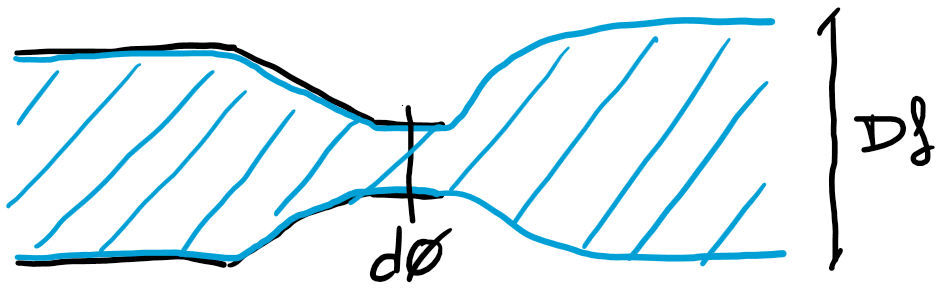
\includegraphics[width = 0.4\textwidth]{gfx/Barus}}\quad
\subfloat[][\emph{Comportamento per fluidi con effeto di rigonfiamento a diverso comportamento elastico}\label{fig:Elasticità}]
{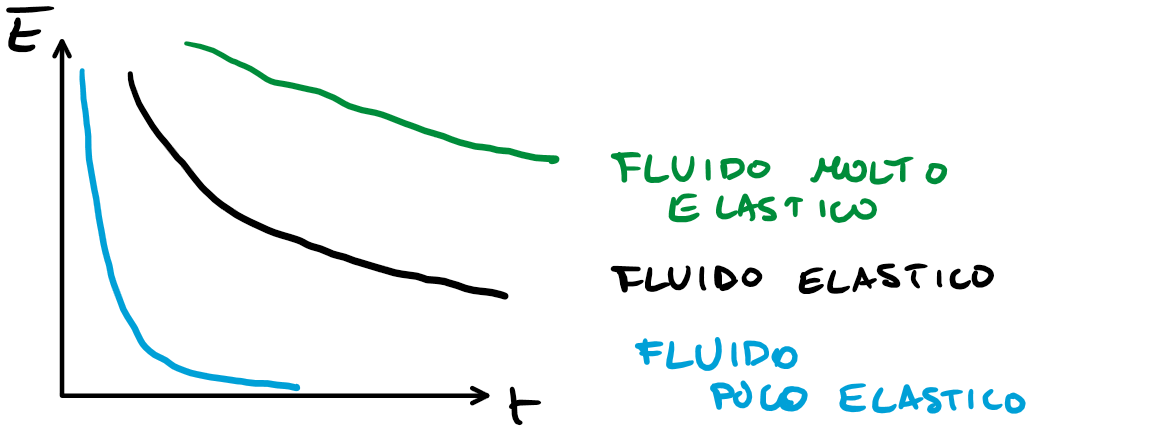
\includegraphics[width = 0.4\textwidth]{gfx/Elasticità}}
\caption{Comportamento dei fluidi con effetto di rigonfiamento dell'estruso}
\label{fig:RigonfiamentoEstruso}
\end{figure}

Si definisce che l'effetto di rigonfiamento:
\begin{equation}
De = \frac{\tau_r}{\tau_p} = \frac{\text{Tempo di rilassamento}}{\text{Tempo caratteristico del processo}}
\end{equation}
Da cui ne deriva:
\begin{description}
\item[$\tau_r \ll \tau_p$] allora $De \approx 0$ allora si dice che il fluido è poco elastico. Comportamento evidenziato al grafico \ref{fig:Elasticità}.
\item[$\tau_r \approx \tau_p$] allora $De \approx 1$ allora si dice che il fluido è più elastico. Sempre evidenziato al grafico \ref{fig:Elasticità}.
\end{description}

\section{Effetti di plasticità}
Un fluido pseudo-plastico possiede forze interne (intermolecolari) che che gli conferiscono il moto al di sotto di un certo valore $\tau$, il fluido non muoverà fino a quando tale valore non verrà superato (Comportamento del fluido di \textbf{Bingham}). 
Sotto lo \eng{Yield stress} il fluido si comporta come solido.
Sopra lo \eng{Yield stress}, lo sforzo cresce con $\dot{\gamma}$.

Il grafico \ref{fig:EffettoPlastico} rappresenta i comportamenti di un fluido puramente pseudo-plastico e il fluido di Bingham.
Entrambi hanno una legge del tipo:
\begin{description}
\item[Fluido di Bingham] $\tau = \tau_y + \eta \dot{\gamma}$
\item[Fluido pseudo-plastico] $\tau = \eta \dot{\gamma}$
\end{description}

\begin{figure}
\centering
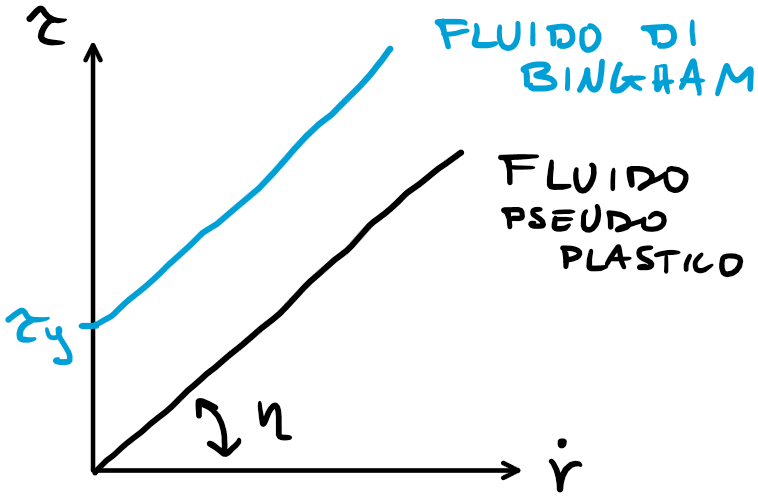
\includegraphics[width = 0.6\textwidth]{gfx/EffettoPlastico}
\caption{Rappresentazione del comportamento sotto l'effetto plastico}
\label{fig:EffettoPlastico}
\end{figure}

\section{Tissotropia}
\begin{figure}
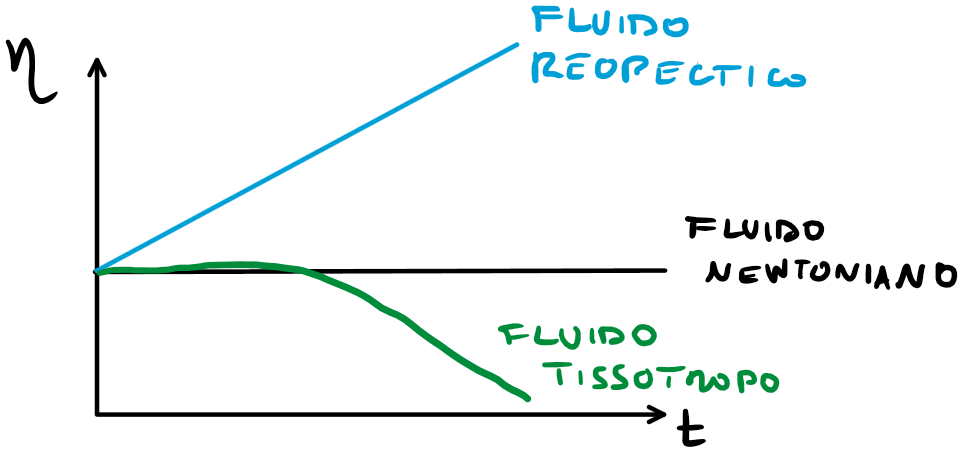
\includegraphics[width = 0.7\textwidth]{gfx/Tissotropia}
\caption{Caratteristica della viscosità in funzione del tempo}
\label{fig:Tissotropia}
\end{figure}
La tissotropia si può presentare in due forme particolari:
\begin{description}
\item[Fluido reopectico] sono quei (pochi) fluidi che aumentano la loro viscosità all'aumentare del tempo.
\item[Fluido tissotropico] sono i fluidi, non newtoniani che diminuiscono la loro viscosità all'aumentare del tempo.
\end{description}

%%%%%%%%%%%%%%%%%%%%%%%%%%%%%%%%%%%%%%%%%%%%%%%%%%%%%%%%%%%%%%%%%%%%%%%%%%%%%%%
\chapter{Reologia (o Reometria)}\label{chp:Reologia}
%%%%%%%%%%%%%%%%%%%%%%%%%%%%%%%%%%%%%%%%%%%%%%%%%%%%%%%%%%%%%%%%%%%%%%%%%%%%%%%
La reologia studia la deformazione di un corpo sotto l'azione di uno sforzo.
I fluidi ideali, liquidi o gassosi che siano, si deformano irreversibilmente. L'energia di deformazione viene dissipata all'interno dei fluido sotto forma di calore, non può essere recuperata alla cessazione dello sforzo. Nella realtà non si trovano né fluidi ideali, né solidi ideali.
Solo pochi liquidi si avvicinano, come comportamento a quello dei liquidi ideali. La maggior parte dei liquidi mostrano reologiacamente un comportamento che li classifica nella regione tra i liquidi e solidi: essi sono sia elastici che viscosi e possono perciò essere definiti "viscoelastici", che possono subire solo sforzi di taglio.

La resistenza di un fluido rispetto ad ogni cambiamento irreversibile dei suoi elementi di volume viene detta viscosità.

\section{La legge della viscosità}
\subsection{La legge di Newton}
La misura della viscosità dei liquidi richiede dapprima la definizione dei parametri che riguardano il flusso. Si potranno poi trovare opportune condizioni per l'esecuzione dei test che consentono la misurazione delle grandezze in modo obbiettivo e riproducibile.
Newton fu il primo a formulare la legge fondamentale della viscometria che descrive il comportamento di flusso di un liquido ideale.
\begin{equation}
\tau = \eta \cdot \dot{\gamma}
\label{eqn:1LeggeNewton}
\end{equation}

\paragraph{Lo sforzo di taglio}
Una forza $\mathbf{F}$ applicata ad un'area $A$ (interfaccia tra il piatto superiore il liquido sottostante) provoca un movimento di scorrimento nello strato liquido. la velocità di flusso che può essere mantenuta per una data forza sarà determinata dalla resistenza interna del liquido, cioè dalla sua viscosità.
\begin{equation}
p = \frac{\mathbf{F}}{A} = \left[\frac{N}{m^2}\right] = \left[Pa\right]
\end{equation}

\section{Le curve di flusso e di viscosità}
la correlazione tra lo sforzo di taglio e gradiente di velocità che definisce il comportamento reologico di un liquido può essere graficamente riportato in un diagramma $t/D$. Il diagramma prende il nome di \textbf{curva di flusso}.
Altro diagramma assai comune è quello che riporta $\eta$ in funzione di $D$ (velocità). Questo diagramma è detto \textbf{Curva di viscosità}.

\section{Fluidi pseudo-plastici}
Molti liquidi mostrano una drastica diminuzione della viscosità quando il gradiente di velocità passa da bassi valori ad alti. In altre parole: quanto più veloce i prodotti farmaceutici vengono spinti, attraverso tubi, o capillari, quanto più velocemente i le vernici vengono spruzzate o pennellate, tanto più diminuisce la viscosità di questi materiali.
Tecnicamente questo significa che sotto l'azione di una determinata forza (o pressione) una maggiore quantità di materiale può essere soggetta allo scorrimento o che può essere ridotto il lavoro meccanico necessario a mantenere una determinata portata.
I materiali che subiscono una fluidificazione dovuta all'aumento del gradiente di velocità sono detti \textbf{pseudo-plastici}.
All'aumentare del gradiente di velocità le particelle allungate sospese nel liquido si orientano nella direzione del moto. Le macromolecole di un fuso o di una soluzione possono disintecciarsi, allungarsi e orientarsi parallelamente alla direzione della forza impressa. L'allineamento delle particelle o delle molecole consente loro di scivolare le une sulle altre e questo comporta una diminuzione della viscosità.
Per la maggior parte dei liquidi la diminuzione di $h$ al crescere di $D$ è irreversibile, magari dopo un certo lasso di tempo, cioè il liquido riacquista la sua elevata viscosità originale per cessazione dello sforzo applicato.


%%%%%%%%%%%%%%%%%%%%%%%%%%%%%%%%%%%%%%%%%%%%%%%%%%%%%%%%%%%%%%%%%%%%%%%%%%%%%%%
\chapter{Misure di Viscosità}\label{chp:MisureViscosità}
%%%%%%%%%%%%%%%%%%%%%%%%%%%%%%%%%%%%%%%%%%%%%%%%%%%%%%%%%%%%%%%%%%%%%%%%%%%%%%%
\section{Viscosimetri rotazionali}
Il principio di funzionamento dei viscosimetri rotazionali con sistema di misura a cilindri coassiali o a piatto cono consente la progettazione di viscosimetri assoluti estremamente versatili.
Nel mercato se ne trovano molti, di vari modelli con alta varietà di prezzo.
Si può pensare al sistema di misura a cilindri coassiali per i viscosimetri rotazionali come derivante dal modello a piatti paralleli di Newton, con la semplice incurvatura dei piatti in due cilindri, l'uno al interno dell'altro. Il campione di liquido riempe l'intercapedine anulare (in visosimetria molto spesso indicata come \eng{gap}) tra i due cilindri può essere sottoposto a taglio. Il moto deve essere laminare al fine di consentire la trattazione matematica del problema.
Si può:
\begin{itemize}
\item Fissare $\tau$ e valutare $D(\dot{\gamma})$: Il cilindro interno, o esterno, impone un definito sforzo di taglio (o momento torcente) mentre l'altro è fermo.
Si può misurare la velocità di rotazione o il gradiente di velocità risultante. Si basano su questo principio i viscosimetri tipo \eng{Krebs-Stormer}.
\item Fissare $\dot{\gamma}$ e trovare $\tau$.
Uno dei cilindro ruota a velocità costante, mentre l'altro è fermo. Si può misurare lo sforzo di taglio risultante o il momento torcente. La maggior parte dei viscosimetri in commercio sfruttano tale principio.
\end{itemize}

\section{Viscosimetro di Couette}
In questo tipo, il cilindro ruota a velocità prefissata mentre la coppia viene misurata da quello interno, attraverso un elemento simile a quello descritto precedentemente (ad esempio una molla).
I viscosimetri di \eng{Couette} sono più stabili di quelli \eng{Searie} per quanto riguarda le forze centrifughe. naturalmente le misure fatte con viscosimetri di tipo diverso danno gli stessi valori di viscosità assoluta per uno stesso fluido.
Se i due viscosimetri sono equipaggiati con ciclindri coassiali di raggio poco diverso, cioè se l'intercapedine in cui sta il fluido è molto sottile, il gradiente $D$ è costante all'interno del fluido, così la viscosità del fluido stesso.
\begin{equation}
\dot{\gamma} = \frac{dv}{dh} = \frac{V}{H} \Rightarrow \tau = \eta \frac{V}{H}
\end{equation}
Per effettuare la misura, si inserisce un cilindro dentro l'altro. Fissato il cilindro esterno, mentre quello interno viene mosso con velocità costante.

\begin{figure}
\centering
\subfloat[][\emph{Schema viscosimetro}\label{fig:Viscosimetro}]
{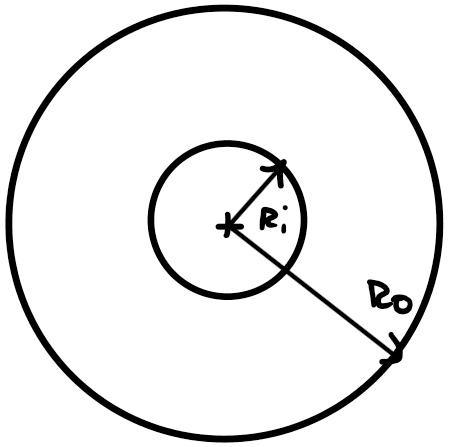
\includegraphics[width = 0.4\textwidth]{gfx/Viscosimetro}}\quad
\subfloat[][\emph{Relazioni calcolate dal viscosimetro}\label{txt:Viscosimetro}]{
\begin{minipage}[b]{0.4\textwidth}
\begin{align*}
H &= R_o - R_i\\
V &= \omega R_i\\
\dot{\gamma} &= \frac{V}{H} = \frac{\omega R_i}{R_o - R_i}\\
\end{align*}
Per ottenere $\tau$ devo trovare il momento torcente:
\begin{align*}
M_{torc} &= \tau 2\pi R_i \cdot \underbrace{l \cdot r_i}_{\text{azione di }\tau} =\\
&= \tau 2\pi \cdot l \cdot R_i^2\\
\Rightarrow \tau &= \frac{M_{torc}}{2\pi l R_i^2} 
\end{align*}
\end{minipage}}
\caption{Funzionamento di un viscosimetro}
\label{exp:Viscosimetro}
\end{figure}

Siccome deve valere che $\eta = \tau / \dot{\gamma}$ se si vuole $\dot{\gamma}$ elevata, bisogna muovere il cilindro interno generando forze centrifughe.
Tuttavia se si accelera troppo il fluido, esso sarà soggetto a instabilità.

\section{Reometro Piatto-Cono}
Nei sistemi di misura piatto-cono (detti \ac{PK}), il problema fondamentale risulta la pulizia.
In certi casi, la pulizia del rotore e della campana dopo aver eseguito dei test è talmente complicata da far orientare la scelta sul sistema piatto-cono, assai più facile da pulire%
\footnote{Soprattutto dopo aver fatto dei test su dei pigmenti}.
alle volte vengono eseguite delle prove su dei campioni contenenti materiali preziosi (in campo dell'elettronica) ed è fondamentale che venga recuperato tutto il campione.
In generale la quantità di campione richiesta per eseguire prove su \ac{PK} è molto inferiore rispetto al sistema a cilindri coassiali.
per la maggior parte dei \ac{PK} sono sufficienti poche gocce di liquido.
I sistemi di misura \ac{PK} trovano la loro principale applicazione nel campi degli alti gradienti di velocità.

Vi sono però alcune importanti limitazioni nell'uso dei sistemi di misura \ac{PK}:
\begin{itemize}
\item L'angolo del cono (in genere si usano angoli variabili tra $0.3\unit{\degree} \div 1.0\unit{\degree}$) fa sì che l'intercapedine tra il piatto e cono varia da zero in punta al cono al valore massimo al raggio $R_o$. Le dispersioni con particelle, anche le più piccole possibili, non sono adatte per la zona vicina alla punta del cono.
\item Le particelle vengno spinte dalla zona della punta verso l'esterno e questo può accadere prima ancora dell'inizio della prova, quando il piano viene avvicinato al cono fino al contatto. Durante la prova, si ha un flusso secondario di particelle in direzione radiale che si sovrappone al flusso principale (circolare). Influenzando negativamente il moto laminare. Una simile situazione tende a rendere ancora di più eterogenei i campioni, falsando la prova.
\item Le particelle più grandi richiedono l'uso di angoli maggiori $1\unit{\degree} \div 3\unit{\degree}$ con conseguenti maggiori effetti negativi del flusso secondario sui risultati del test.
\item I sistemi \ac{PK} sono influenzati dalle forze normali che sono il risultato della risposta elastica dei campioni viscoelastici soggetti a taglio.
Queste forze normali possono trascinare elementi di volume fuori del gap angolare e farli arrampicare sul bordo esterno del cono, In tale situazione si ha spaccamento del campione verso la metà del gap angolare. Ciò è un problema che disturba fortemente la misura.
Un'indicazione della presenza di questo inconveniente è il formarsi di una cresta sempre più grande sul bordo del cono. Spesso si arriva addirittura a vedere la spaccatura del campione guardando da vicino la rotazione del cono.
\end{itemize} 

\begin{figure}
\centering
\subfloat[][\emph{Funzionamento del cono (1), caso di separazione del campione (2)}\label{fig:PK}]
{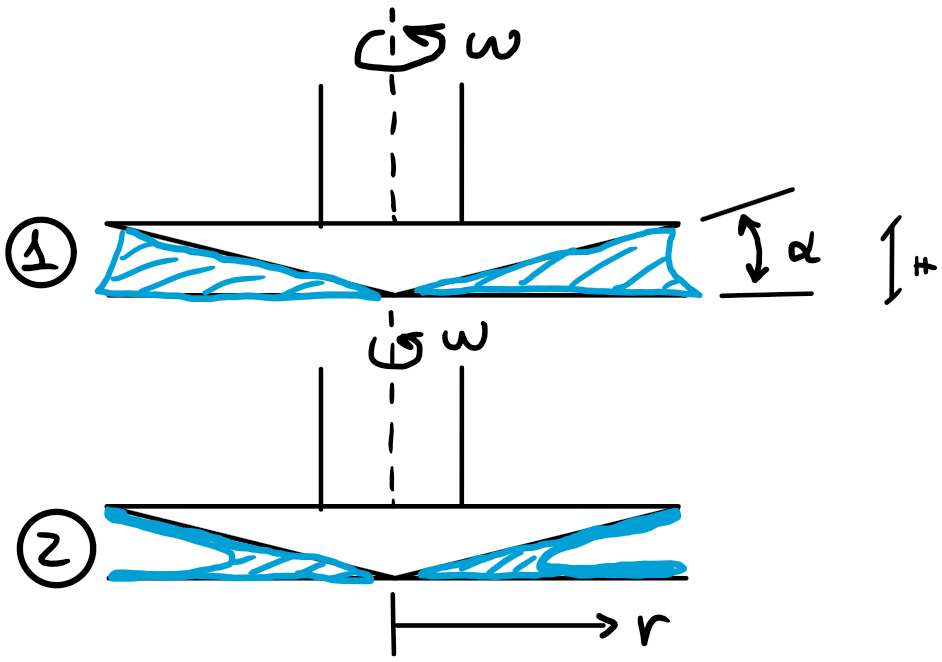
\includegraphics[width = 0.4\textwidth]{gfx/PK}}\quad
\subfloat[][\emph{Grafico ottenuto dal test}\label{fig:PK_graph}]
{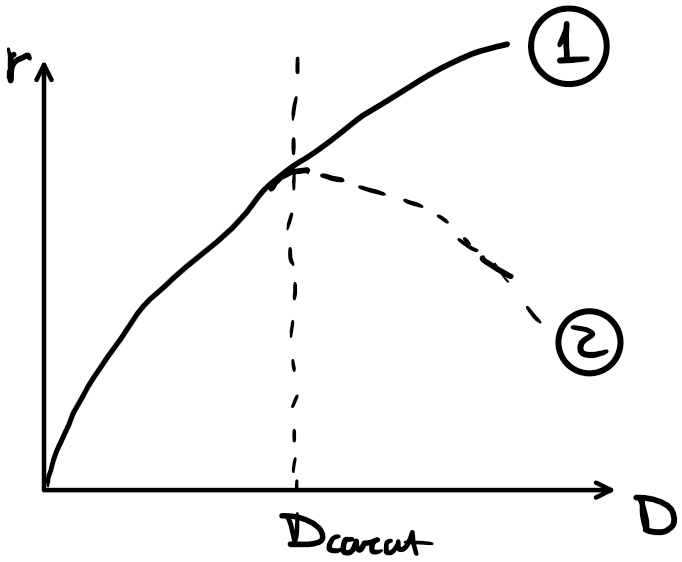
\includegraphics[width = 0.4\textwidth]{gfx/PK_graph}}
\caption{Schematizzazione dei test eseguiti tramite sistema \ac{PK}}
\label{fig:TestPK}
\end{figure}
Allora i calcoli che permettono di ottenere una valutazione della viscosità diventano:
\begin{align}
v &= \omega r \frac{z}{\alpha r}\\
&= \frac{\omega z}{\alpha}\\
\Rightarrow \dot{\gamma} &= \frac{dv}{dz} = \frac{\omega}{\alpha}\: cost.
\end{align}
Dunque:
\begin{equation}
\tau = \eta \frac{\omega}{\alpha}
\end{equation}
\begin{align}
M_t &= \int_0^R \tau 2\pi r^2 dr =\\
&= 2\pi \eta \frac{\omega}{\alpha} \frac{R^3}{3}\\
\Rightarrow \tau &= \frac{3 M_t}{2\pi R^3}
\end{align}
Da cui in fine si ottiene la viscosità sostituendo in
\begin{equation}
\eta = \frac{\tau}{\dot{\gamma}}
\end{equation}

\section{Reometro Piatto-Piatto}
\begin{figure}
\centering
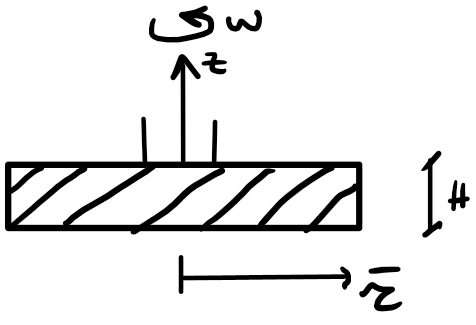
\includegraphics[width = 0.5\textwidth]{gfx/PiattoPiatto}
\caption{Schema del rotore per uno strumento piatto piatto}
\label{fig:PiattoPiatto}
\end{figure}

Nella figura \ref{fig:PiattoPiatto} viene rappresentato il rotore dello strumento per la misura della viscosità.
La relazione che ci permetterà di ottenere la viscosità sarà:
\begin{equation}
v(r,z) = \omega r \frac{z}{H} =%
\begin{cases}
\omega r & se z = H\\
0 & se z = 0
\end{cases}
\end{equation}
Da cui allora:
\begin{equation}
\dot{\gamma} = \frac{dv}{dz} = \frac{\omega r}{H}
\end{equation}
\begin{equation}
\dot{\gamma}_R = \frac{dv}{dz} = \frac{\omega R}{H}
\end{equation}
Calcoliamo il momento torcente
\begin{equation}
M_t = \int_0^R{\tau 2\pi r^2 dr}
\end{equation}
Ipotizzando che si sita analizzando un fluido newtoniano.
\begin{equation}
\eta \frac{\omega}{H} 2\pi \int_0^R{r^3 dr} =%
2\pi \eta \frac{\omega}{H} \frac{R^4}{4}
\end{equation}
Da cui
\begin{equation}
\frac{\pi}{2} \eta \frac{\omega}{H} R^4
\end{equation}
Notiamo che
\begin{equation}
\frac{\pi}{2} \underbrace{\eta \frac{\omega R}{H}}_{\tau} R^3 = \frac{\pi}{2} \tau_R R^3
\end{equation}
Invertendo l'equazione di definizione del momento torcente:
\begin{equation}
\tau_R = \frac{M_t 2}{\pi R^3}
\end{equation}
Da cui finalmente si ottiene la densità, sempre ricordando che tutti questi ragionamenti valgono per un fluido newtoniano:
\begin{equation}
\eta = \frac{\tau_R}{\dot{\gamma}_R}
\end{equation}

\section{Viscosimetro capillare}
L'utilità di questo tipo di misuratore, di fatto è la controparte del \ac{MFI}.
In quanto in termini di:
\begin{description}
\item[Pressione] \ac{MFI} controllando la pressione da cui si misura la portata di fluido;
\item[Portata di flusso] Viscosimetria capillare: si controlla la portata e si misura la pressione.
\end{description}

Il reometro è costituito da una camera cilindrica in cui viene caricato il materiale che successivamente viene estruso attraverso l'ugello. Viene spinto da un pistone che scorre verso il basso.
Il materiale viene tenuto fuso grazie ad un forno che circonda la camera, mantenendola ad una temperatura $T$ impostata.
Durante la misura, il pistone scende secondo velocità impostata e, contemporaneamente, ad intervalli prestabiliti misura il valore della forza necessaria all'estrusione del materiale.
La misura avviene grazie ad una cella di carico che lavora in un range $0 \div 2000\unit{\N}$, alloggiata nella testa del pistone.
Al fine di determinare le relazioni che legano: lo sforzo di taglio, il gradiente di velocità e le grandezze misurabili nel sistema, è necessario studiare il flusso in un capillare.
Partendo dalla figura \ref{fig:Capillare}, si può scrivere il bilancio delle forze sul cilindro di fluido di raggio $R$ e lunghezza $L$
\begin{equation}
(P_1 - P_2)\pi R^2 = 2\pi RL \tau_W
\end{equation}
da cui
\begin{equation}
\tau_W = \frac{\Delta P R}{2 L}
\end{equation}

\begin{figure}
\centering
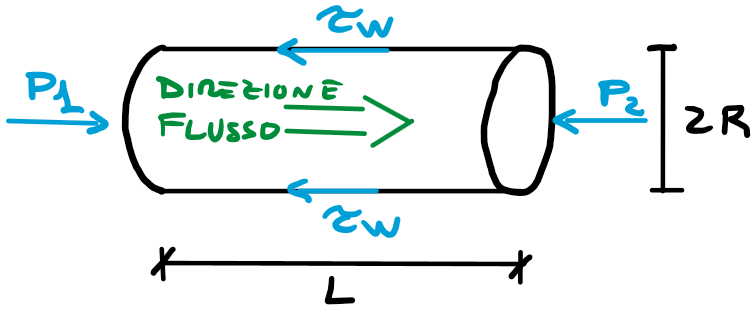
\includegraphics[width = \textwidth]{gfx/Capillare}
\caption{Indicazioni dei parametri del sistema per la misura capillare}
\label{fig:Capillare}
\end{figure}

Nel caso che il bilancio venga scritto in corrispondenza di un raggio generico, si avrebbe:
\begin{equation}
\tau = \frac{\Delta P r}{2 L}
\end{equation}

Per poter determinare le relazioni tra le varie grandezze, l'approccio conveniente è quello di introdurre un'equazione costitutiva semplice%
\footnote{Ad esempio quella dei fluidi newtoniani.}
cercando poi una correzione che permetta di estendere le equazioni trovate a qualunque tipo di fluido.

Introduciamo l'equazione costitutiva relativa ad un fluido newtoniano sostituendola allo sforzo di taglio:
\begin{equation}
\eta \frac{d V_z}{dr} = \frac{\Delta P r}{2 L}
\end{equation}
questa equazione differenziale a variabili separabili ci permette di determinare l'espressione del profilo di velocità in funzione del ragio. Separando le variabili e considerando che in $V_z(R) = 0$:
\begin{equation}
\int_0^{V_z(r)}{\frac{2\eta L}{\Delta P} dV_z} = \int_R^r rdr
\end{equation}
da cui:
\begin{equation}
V_z(r) = \frac{\Delta P}{4 \eta L} R^2 \left[1 - \left(\frac{r}{R}\right)^2\right] 
\end{equation}

La portata $Q$ può essere ottenuta integrando il profilo di velocità sull'area della sezione di passaggio è data da:
\begin{equation}
Q = \frac{\Delta P \pi R^4}{8 \eta L} \Leftarrow%
\frac{\pi R^3}{4 \eta} \tau_{\omega} =%
\frac{\pi R^3}{4 \eta} \frac{\overbrace{P R}^{\tau_{\omega}}}{2L}
\end{equation}

Dall'equazione dello sforzo di taglio alla parete $\tau_W$ è possibile calcolare lo sforzo di taglio alla parete:
\begin{equation}
\dot{\gamma}_W = \frac{\tau_W}{\eta} = \frac{\Delta P R}{2 L}
\end{equation}
Sostituendo in questa, l'equazione di $\Delta P$ ricavabile dalla definizione della portata:
\begin{equation}
\dot{\gamma}_W = \frac{4Q}{\pi R^3}
\end{equation}
Quando il fluido ha comportamento non newtoniano, è necessario introdurre due correzioni:
\begin{enumerate}
\item Correzione di Rabinowitsch;
\item Correzione di Bagley.
\end{enumerate}

\paragraph{Melt Flow Index}
Riprendendo ciò che era già stato visto al capitolo dedicato.
%TODO aggiungere il riferimento al capitolo\eng{•}

\begin{equation}
\text{Portata} = \frac{\text{Pressione}}{A}
\end{equation}
con:
\begin{equation}
A = \frac{\pi D^2}{4}
\end{equation}
Si considera allora:
\begin{description}
\item[MFI alto] allora $\mu \downarrow$ con circa
$MFI \approx 25 \div 50 \unit{\g/10\min}$
\item[MFI basso] allora $\mu \uparrow$ con circa
$MFI \approx 0.5 \div 5 \unit{\g/10\min}$
\end{description}

\begin{figure}
\centering
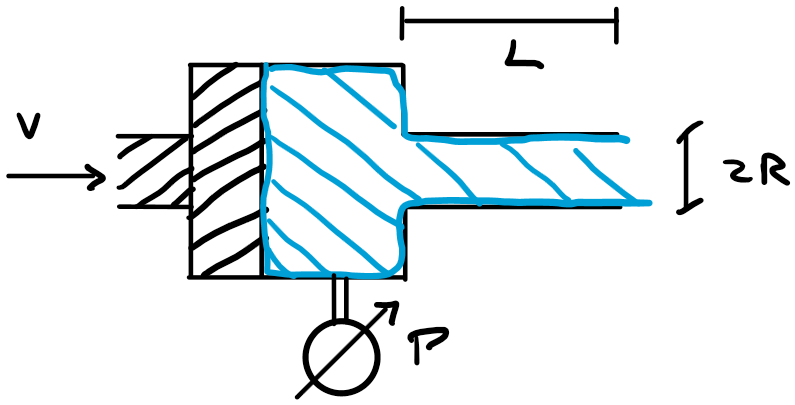
\includegraphics[width = 0.5\textwidth]{gfx/CorrezioneCapillare}
\caption{Descrizione del viscosimetro capillare con le correzioni per i fluidi non newtoniani}\label{fig:CorrezioneCapillare}
\end{figure}

\subsection{Correzione di Rabinowitsch}
\begin{equation}
\dot{\gamma}_W = \frac{4 Q}{\pi R^3} + \ldots
\end{equation}

\subsection{Correzione di Mooney}
Corregge lo scorrimento per adesione alle pareti che non veniva considerato nella correzione di Rabinowitsch.
Per eseguire più velocemente nell'esecuzione della prova si può usare un lubrificante. Saranno però necessarie più misure per raggi diversi.
Allora:
\begin{equation}
\dot{\gamma}_W  = \frac{4 Q}{\pi R^3} = \dot{\gamma}_N
\end{equation}
Sapendo che:
\begin{equation}
\dot{\gamma} = \frac{dv}{dr} \quad \dot{\gamma}_W = \frac{dv}{dr}\Big|_{r = R}
\end{equation}
Dal moto di Poiseville si può descrivere:
\begin{equation}
\tau = - \frac{r}{R}\tau_W \quad \tau_W = \frac{PR}{2L}
\end{equation}
allora si può andare a definire la portata per la figura \ref{fig:CorrezioneCapillare}:
\begin{equation}
\begin{split}
Q &= \int_A{v(r) dA} = \int_0^R{v(r) \underbrace{2\pi r dr}_{dA}} = 2\pi \int_0^R{v(r) r dr} =\\
&= 2\pi \left[v(r) \frac{r^2}{2}\right]_0^R - \int_0^R{\frac{dv}{dr}\frac{r^2}{2}dr} =\\
&= 2\pi \left[v(R)\frac{R^2}{2} - v(0)\frac{0^2}{2}\right] - \int_0^R{\dot{\gamma}\frac{r^2}{2}dr} =\\
&= -\pi \int_0^R{\dot{\gamma}r^2 dr} \Rightarrow \underbrace{\left[r = \frac{\tau}{\tau_W}R\right]}_{\text{cambio variabili}} \Rightarrow\\
&\Rightarrow \pi \int_{0 \mid r = 0}^{-\tau_W \mid r=R \Rightarrow \tau = -\tau_W}{\dot{\gamma}(\tau)\frac{\tau^2}{\tau_W^2}R^2\frac{R}{\tau_W}d\tau}=\\
&= \pi \frac{R^3}{\tau_W^3}\int_0^{-\tau_W}{\dot{\gamma}(\tau) \tau^2 d\tau}
\end{split}
\end{equation}
Da cui
\begin{equation}
\begin{split}
\frac{dQ}{d\tau_W} &= -\frac{3}{\tau_W^4}\pi R^3%
\int_0^{-\tau_W}{\dot{\gamma}(\tau)\tau^2 d\tau} - \frac{\pi R^3}{\tau_W^3} \dot{\gamma}(-\tau_W)\tau_W^3\\
&= -\frac{3\pi R^3}{\tau_W^4}\int_0^{-\tau_W}{\dot{\gamma}\tau^2 d\tau} + \frac{\pi R^3}{\tau_W}\dot{\gamma}_W
\end{split}
\end{equation}
Per cui:
\begin{equation}
Q = \frac{\pi R^3}{\tau_W^3}\int_0^{-\tau_W}{\dot{\gamma}(\tau)\tau^2 d\tau}
\end{equation}
Svolgendo l'integrale si arriva ad ottenere:
\begin{equation}
\frac{Q \tau_W^3}{\pi R^3}
\end{equation}
Allora:
\begin{equation}
\begin{split}
\frac{dQ}{d\tau_W} &= - \frac{3\pi R^3}{\tau_W^4} \frac{Q \tau_W^3}{\pi R^3} + \frac{\pi R^3}{\tau_w}\dot{\gamma}_W\\
\frac{dQ}{d\tau_w} &= -\frac{3Q}{\tau_W} + \frac{\pi R^3}{\tau_W}\dot{\gamma}_W
\end{split}
\end{equation}
Imponiamo la pre-moltiplicazione per $4/\pi R^3$ :
\begin{equation}
\frac{4}{\pi R^3}\frac{dQ}{d\tau_w} = \left[-\frac{3Q}{\tau_W}+\frac{\pi R^3}{\tau_w}\dot{\gamma}_W\right]\frac{4}{\pi R^3}
\end{equation}
Inoltre
\begin{equation}
\frac{\dot{\gamma}_W}{d\tau_W} = -\frac{3 Q \dot{\gamma}_N}{\tau_W} + \frac{4 \dot{\gamma}_W}{\tau_W}
\end{equation}
Da cui:
\begin{equation}
\begin{split}
\dot{\gamma}_W &= \frac{\tau_W}{4}\left[\frac{3}{\tau_W}\dot{\gamma}_W + \frac{d\dot{\gamma}_W}{d\tau_W}\right]\\
\dot{\gamma}_W &= \gamma_W \left[\frac{3}{4} + \frac{1}{4}\frac{\tau_W}{\dot{\gamma}_N}\frac{d\dot{\gamma}_N}{d\tau_W}\right]
\end{split}
\end{equation}
Piccola nota sull'ultimo termine dell'equazione precedente:
\begin{equation}
\frac{\tau_W}{\dot{\gamma}_N} \frac{d\dot{\gamma}_N}{d\tau_W} = \frac{\frac{d\dot{\gamma}_N}{\dot{\gamma}_N}}{\frac{d\tau_W}{\tau_W}} = \frac{d \ln\dot{\gamma}_N}{d\ln\tau_W}
\end{equation}
Dunque:
\begin{equation}
\dot{\gamma}_W = \dot{\gamma}_N\left[\frac{3}{4} + \frac{1}{4} \frac{d \ln\dot{\gamma}_N}{d\ln\tau_W}\right]
\end{equation}
Seguendo la \textbf{legge di potenza} si può scrivere:
\begin{equation}
\frac{d \ln\dot{\gamma}_N}{d\ln\tau_W} = \frac{1}{n} \Rightarrow \text{Fattore di Rabinowitch} \Rightarrow \frac{3n+1}{4n}
\end{equation}
In fine:
\begin{equation}
\dot{\gamma_W} = \frac{4Q}{\pi R^3}\frac{3n+1}{4n}
\end{equation}
Per definire correttamente il rapporto $\frac{d \ln\dot{\gamma}_N}{d\ln\tau_W}$ si può ottenere in maniera sperimentale per singoli punti. Da cui poi si osserva un comportamento descritto come: $\frac{3n+1}{4n}$ come in figura \ref{fig:CorrezioneDoppioLog}.

\begin{figure}
\centering
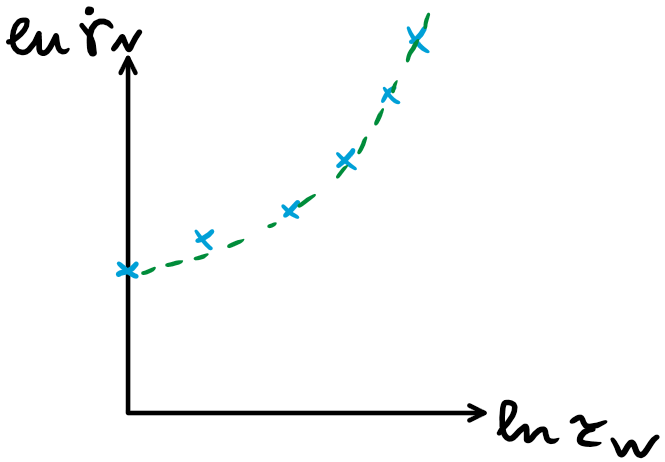
\includegraphics[width = 0.7\textwidth]{gfx/CorrezioneDoppioLog}
\caption{Descrizione del fattore di Rabinowitch ottenuto sperimentalmente}
\label{fig:CorrezioneDoppioLog}
\end{figure}

\subsection{Correzione di Bagley}
COme già visto, l'equazione dello sforzo di taglio è la seguente:
\begin{equation}
\tau_W = \frac{\Delta P R}{2L} \quad \tau_W =\frac{PR}{2L}
\end{equation}
Dove con $\Delta P$ sono le perdite di carico totali relative al processo di estrusione.
Alla base di questa equazione, c'è l'ipotesi di poter trascurare i seguenti fenomeni:
\begin{itemize}
\item La possibilità di un non perfetto accoppiamento tra pistone matrice.
\item Gli attriti derivanti dal moto nella camera.
\item Le perdite di carico in ingresso, dovute al riarrangiamento del profilo di velocità che si ha all'entrata dell'ugello.
Tale riarrangiamento è dovuto al restringimento del filetto fluido delle dimensioni della matrice a quelle del capillare.
\item Altro contributo a tali perdite è il gradiente di pressione maggiore che si ha nella prima parte del capillare, derivante da un flusso non ancora perfettamente sviluppato.
\end{itemize}

Mentre i primi tre contributi sono senz'altro trascurabili, altrettanto non si può dire per gli ultimi due. Per tener conto di questi effetti, viene introdotta la correzione di \eng{Bagley}.
Si tratta di valutare le perdite di carico totali per ugelli con diversi rapporti $L/R$ ad un determinato valore di gradiente di velocità.
Riportando su un grafico \ref{fig:Bagley} i valori trovati, si estrapola il valore delle perdite di carico per $L/R = 0$%
\footnote{Ovvero il punto di incontro della retta con l'asse delle ordinate},
assumendo che questo coincida con la somma delle perdite di carico in entrata ed in uscita a quel determinato gradiente di velocità.
L'operazione viene poi ripetuta per ogni gradiente di velocità, ottenendo così un vettore di perdite di carico.

\begin{figure}
\centering
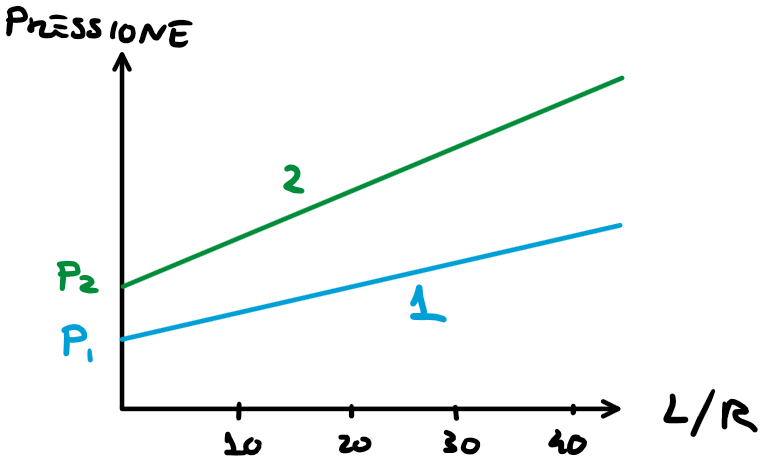
\includegraphics[width = 0.7\textwidth]{gfx/Bagley}
\caption{Rette di Bagley}
\label{fig:Bagley}
\end{figure}

Allora il valore dello sforzo di taglio:
\begin{equation}
\tau_W = \frac{PR}{2(L + L^*)} = \frac{PR}{2(L + eR)}
\end{equation}
Le perdite saranno:
\begin{equation}
P = \frac{\tau_W 2(L + eR)}{R}
\end{equation}
Allora ne risulta
\begin{equation}
\dot{\gamma}_N = \frac{4Q}{\pi R^3}
\end{equation}
Ipotizzando  che $Q$ e $R$ siano costanti allora anche $\dot{\gamma}_N$ sarà costante.
Dato che $\tau_W = \eta \cdot \dot{\gamma}_N$, allora anche $\tau_W$ sarà costante.
